\documentclass[a4paper,10pt]{report}
\usepackage[utf8]{inputenc}
\usepackage{graphicx}
\usepackage{verbatim}
\usepackage{ctable} % for \specialrule command

%\usepackage[a4paper, total={6in, 8in}]{geometry}
% Title Page
\title{\textbf{OPTICAL COMMUNICATION COMPONENTS \\ Lab 8}}
\author{Nicola Simoni, Tadewos Somano, Melkamsew Tenaw}
\date{University of Brescia, Faculty of Engineering\\A.Y. 2013-2014}


\begin{document}
\maketitle


%%%%%%%%%%%%%%%%%%%%%%%%%%%%%%%%%%%%%%%%%%%%%%%%%%%%%%%%%%%%%%%%%%%%%%%%%%%%%%%%%%%%%%%%%%%%%
\section*{Question 1}
We use a pseudo random binary sequence generator. Its output is split in two parts: one goes through a transmission system and
ends into an error detector, the other, instead, is directly connected to the error detector.
We estimate the BER by looking at the eye diagram: the value is 0.0227.
In Figure \ref{q1_2} is shown the plot of the eye.

\begin{figure}[!ht]
   \centering
   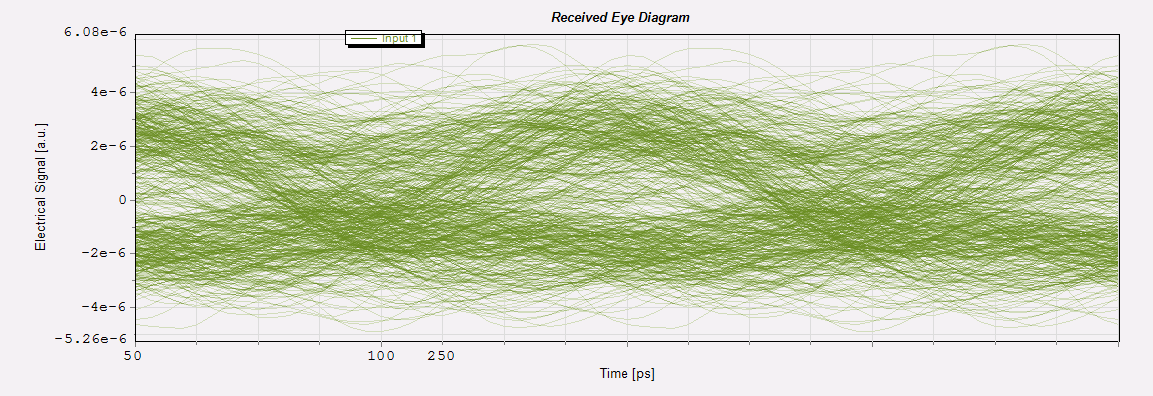
\includegraphics[width=11cm]{q1_2.png}\\
   \caption{Eye diagram.}
   \label{q1_2}
\end{figure}

The exact BER, computed with the error detector, is 0.0293. We can observe that the real value is higher respect to the estimated one.
In Figure \ref{q1_1} is shown a snapshot of the received sequence.

\begin{figure}[!ht]
   \centering
   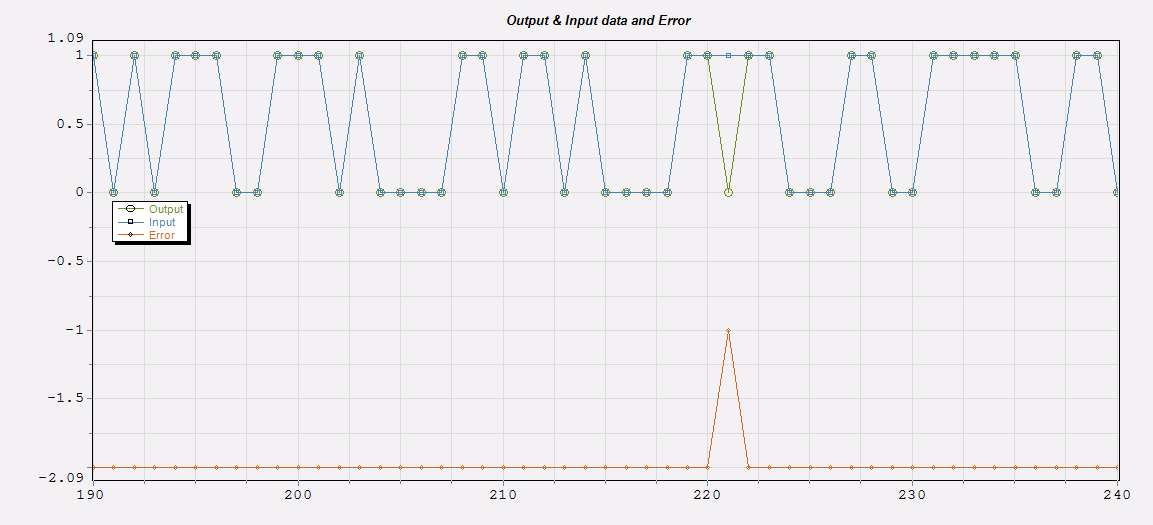
\includegraphics[width=11cm]{q1_1.png}\\
   \caption{Received sequence.}
   \label{q1_1}
\end{figure}

The two BER values are different because the estimation on the eye diagram is done in a statistical way, by assuming that the distribution
of ``0s'' and ``1s'' is Gaussian.
In order to have the convergence between the two results, we need to have an actual Gaussian distribution, and this happens when the transmitted
sequence is sufficiently long. This means that for example, if we have a BER of $10^{-9}$, to detect one error, on average,
we need to transmit at least $10^{9}$ bits.

%%%%%%%%%%%%%%%%%%%%%%%%%%%%%%%%%%%%%%%%%%%%%%%%%%%%%%%%%%%%%%%%%%%%%%%%%%%%%%%%%%%%%%%%%%%%%
\section*{Question 2}
In a computer simulation the BER is not obtained by counting the received and the error bits because of the computation complexity.
In fact, instead of comparing each bit, if we assume that the distribution of the bits is Gaussian, the BER can be calculated more easily.

%%%%%%%%%%%%%%%%%%%%%%%%%%%%%%%%%%%%%%%%%%%%%%%%%%%%%%%%%%%%%%%%%%%%%%%%%%%%%%%%%%%%%%%%%%%%%
\section*{Exercise 1}
We run the simulation and we plot the amplitude histogram of the received signal.
The initial parameters are the following:
\begin{itemize}
 \item Attenuation: 24 dB
 \item Bandwidth: 10 GHz
 \item Length: 50 Km
 \item Average power: 1 mW
 \item Extinction ratio: 30 dB
\end{itemize}

In Figure \ref{ex1_1} is shown the result: the estimated BER is 0.0227.
\begin{figure}[!ht]
   \centering
   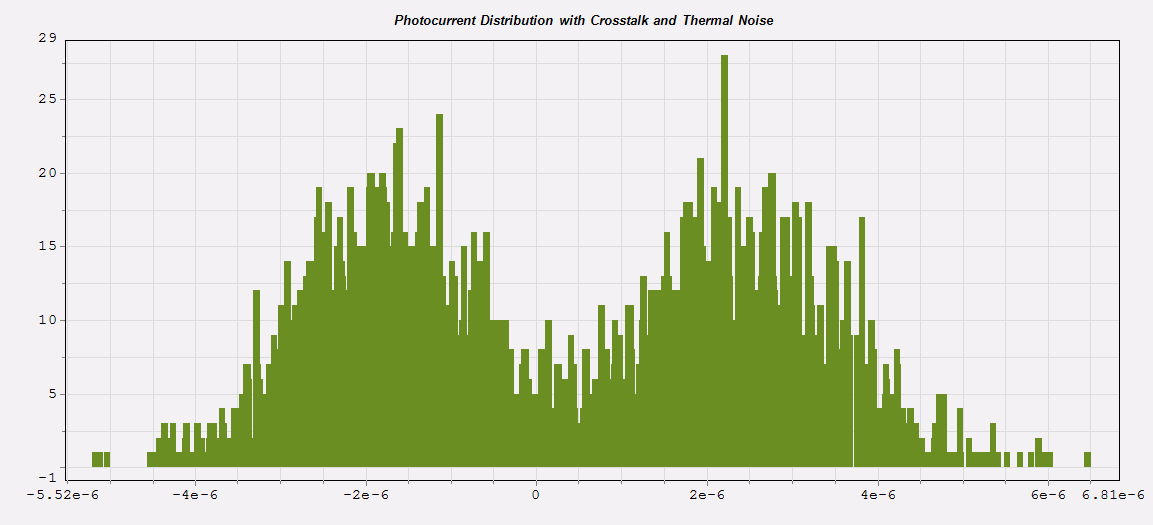
\includegraphics[width=11cm]{ex1_1.png}\\
   \caption{Histogram, $\alpha = 24$ dB.}
   \label{ex1_1}
\end{figure}

We decrease the attenuation and we compare the histograms of the signals.
In Figure \ref{ex1_2} is shown the result obtained using an attenuation of 20 dB.
We can observe that the two peaks are well separated: the estimated BER is $1.054 \cdot 10^{-5}$.

\begin{figure}[!ht]
   \centering
   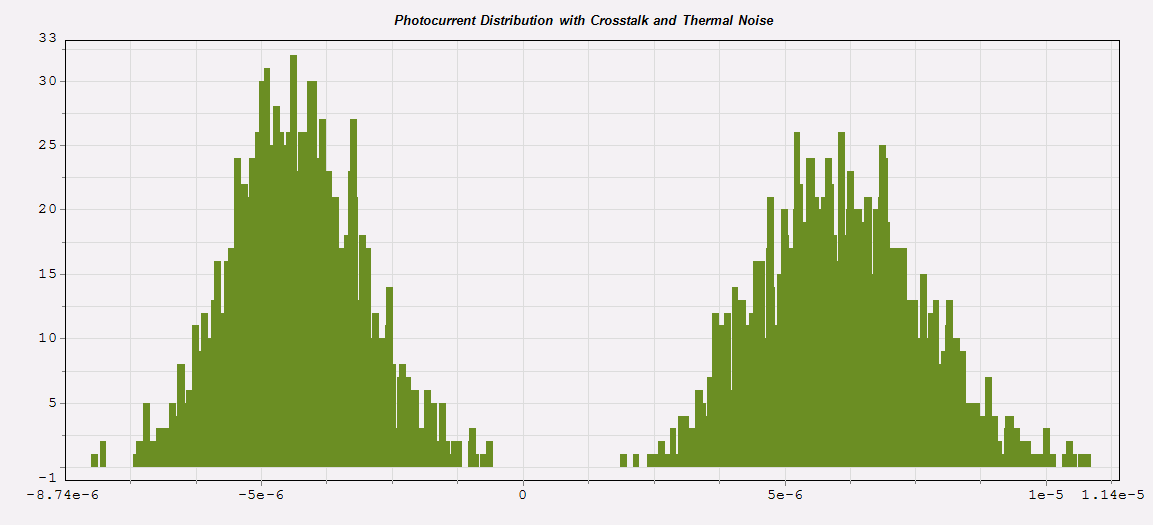
\includegraphics[width=11cm]{ex1_2.png}\\
   \caption{Histogram, $\alpha = 20$ dB.}
   \label{ex1_2}
\end{figure}


In Figure \ref{ex1_3} is shown the result with an attenuation of 12 dB: the estimated BER is $9.806 \cdot 10^{-14}$.

\begin{figure}[!ht]
   \centering
   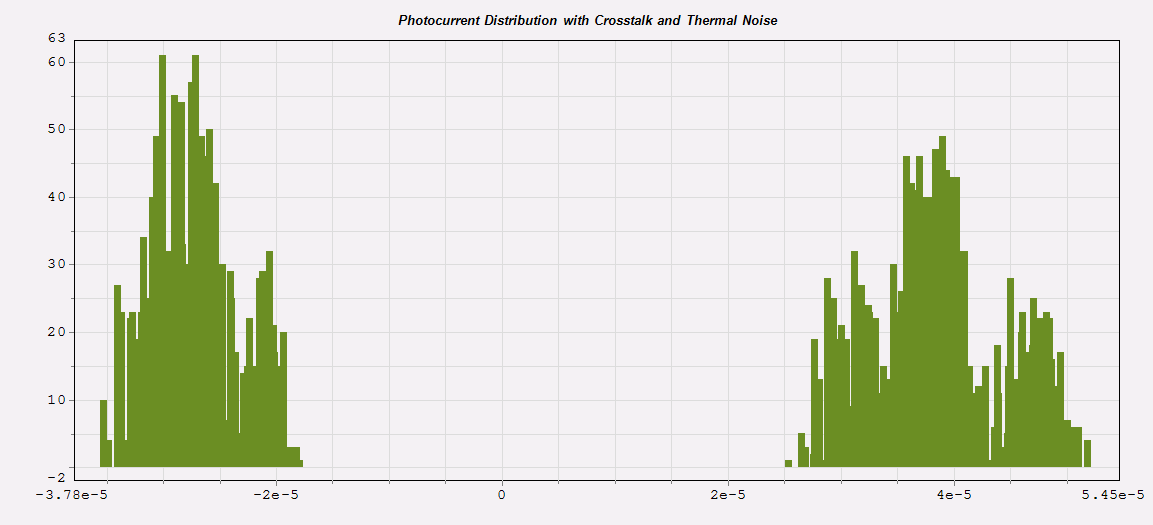
\includegraphics[width=11cm]{ex1_3.png}\\
   \caption{Histogram, $\alpha = 12$ dB.}
   \label{ex1_3}
\end{figure}

In Figure \ref{ex1_4} is shown the result with an attenuation of 6 dB: the estimated BER is $2.671 \cdot 10^{-14}$.

\begin{figure}[!ht]
   \centering
   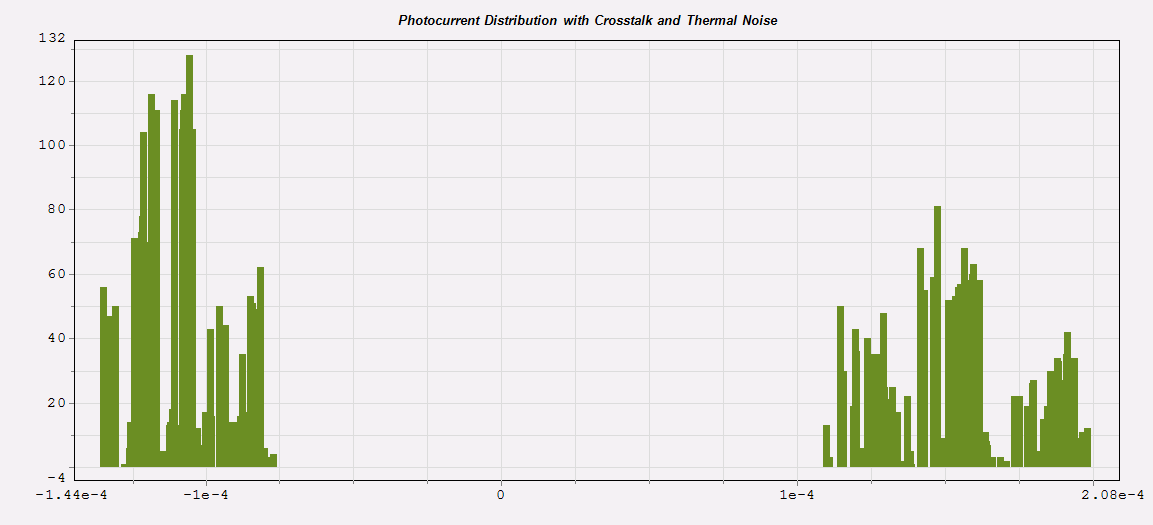
\includegraphics[width=11cm]{ex1_4.png}\\
   \caption{Histogram, $\alpha = 6$ dB.}
   \label{ex1_4}
\end{figure}


We can deduce that reducing the attenuation also the BER decreases. In fact, by having less attenuation, we obtain a better
representation of the signal at the receiver, and so it is easier to distinguish the values ``0'' and ``1''. This is confirmed
also by the histograms: when the attenuation decreases, the distribution of the two amplitudes is better
discriminated and the percentage of samples that fall into the respective voltage bin increases.

\newpage
%%%%%%%%%%%%%%%%%%%%%%%%%%%%%%%%%%%%%%%%%%%%%%%%%%%%%%%%%%%%%%%%%%%%%%%%%%%%%%%%%%%%%%%%%%%%%
\section*{Exercise 2}
We repeat the same simulation of Exercise 1, but varying the bandwidth of the electrical filter after the receiver.
In Figure \ref{ex2_1} is shown the result with a bandwidth of 5 GHz. The estimated BER is $6.27 \cdot 10^{-3}$.

The BER value is better than the one obtained with the same attenuation and a bandwidth of 10 GHz, because the bit-rate is 10 Gb/s
and the optimal value of the bandwidth is around 7 GHz. By using 10 GHz we obtain a worsen BER because we introduce more noise.

\begin{figure}[!ht]
   \centering
   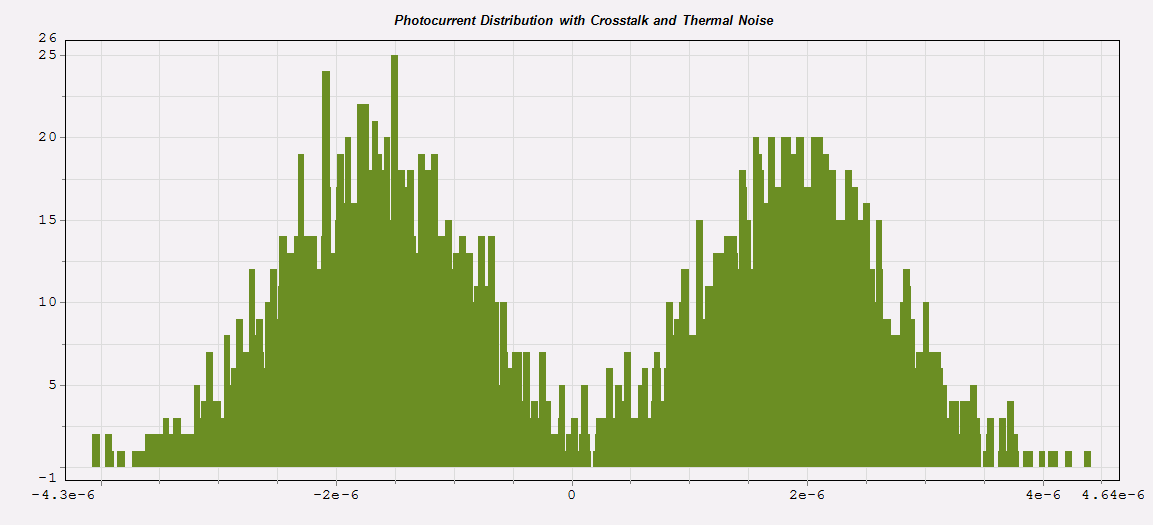
\includegraphics[width=11cm]{ex2_1.png}\\
   \caption{Histogram, BW=5 GHz.}
   \label{ex2_1}
\end{figure}

In Figure \ref{ex2_2} is shown the result with a bandwidth of 2.5 GHz: the estimated BER is $3.69 \cdot 10^{-2}$.

\begin{figure}[!ht]
   \centering
   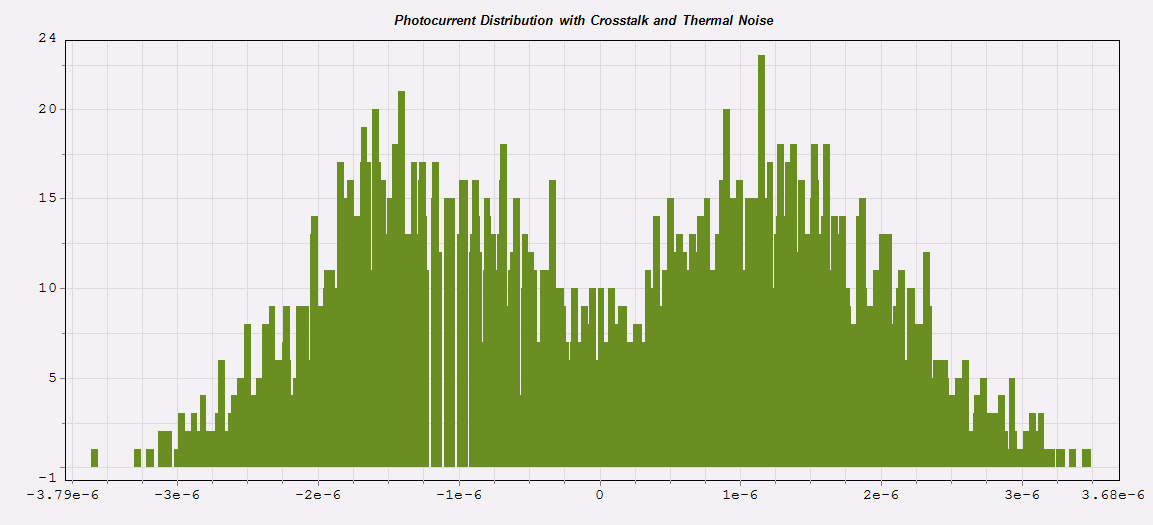
\includegraphics[width=11cm]{ex2_2.png}\\
   \caption{Histogram, BW=2.5 GHz.}
   \label{ex2_2}
\end{figure}

In Figure \ref{ex2_3} is shown the result with a bandwidth of 1 GHz: the estimated BER is 0.209.

\begin{figure}[!ht]
   \centering
   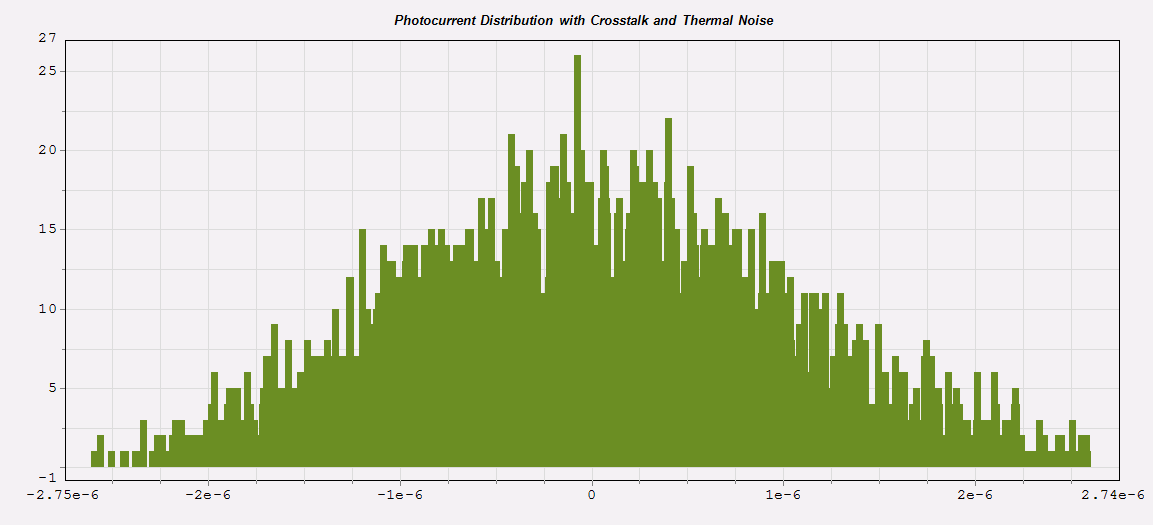
\includegraphics[width=11cm]{ex2_3.png}\\
   \caption{Histogram, BW=1 GHz.}
   \label{ex2_3}
\end{figure}

We can observe that, if we decrease the bandwidth, the BER increases. This is due to the fact that, by decreasing the bandwidth of the filter
after the receiver, some of the frequencies are filtered out and so we have a distortion of the signal.

\newpage
%%%%%%%%%%%%%%%%%%%%%%%%%%%%%%%%%%%%%%%%%%%%%%%%%%%%%%%%%%%%%%%%%%%%%%%%%%%%%%%%%%%%%%%%%%%%%
\section*{Exercise 3}
Now we modify the other parameters and we observe their effect on the BER.
We start by doubling the transmitted power: we set it to 2 mW. In Figure \ref{ex3_1} is shown the result.
As we use more power, it is easier to discriminate between the values ``0'' and ``1'' at the receiver: the estimate BER is $1.52 \cdot 10^{-4}$.

\begin{figure}[!ht]
   \centering
   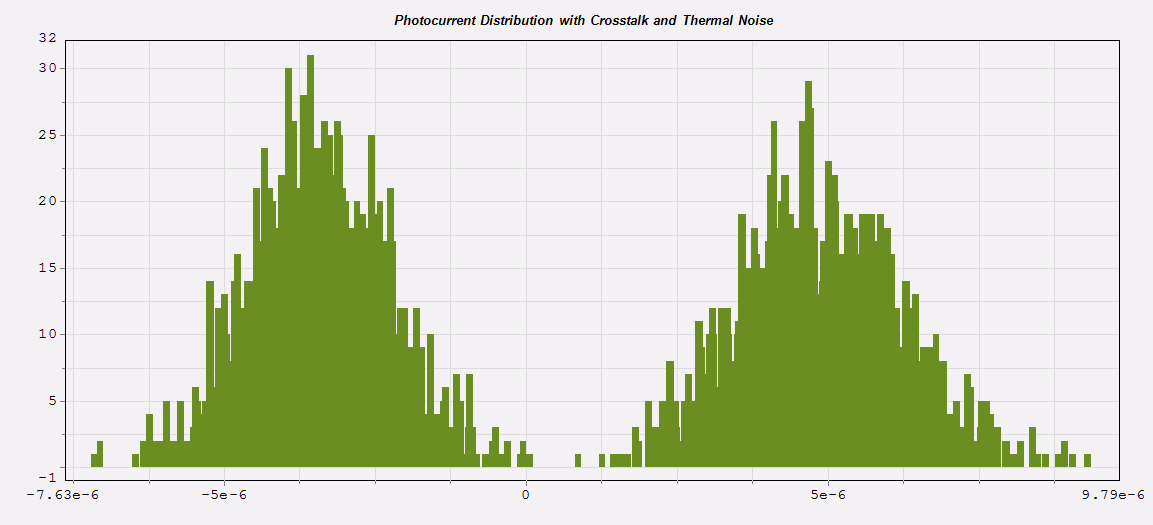
\includegraphics[width=11cm]{ex3_1.png}\\
   \caption{Histogram, P=2 mW.}
   \label{ex3_1}
\end{figure}

Now we increase the length of the transmission link: we set it at 100 Km.
In Figure \ref{ex3_2} is shown the histogram. The estimated BER is 0.424: as we increased the length, the signal is more attenuated
and at the receiver the discrimination is more difficult.

\begin{figure}[!ht]
   \centering
   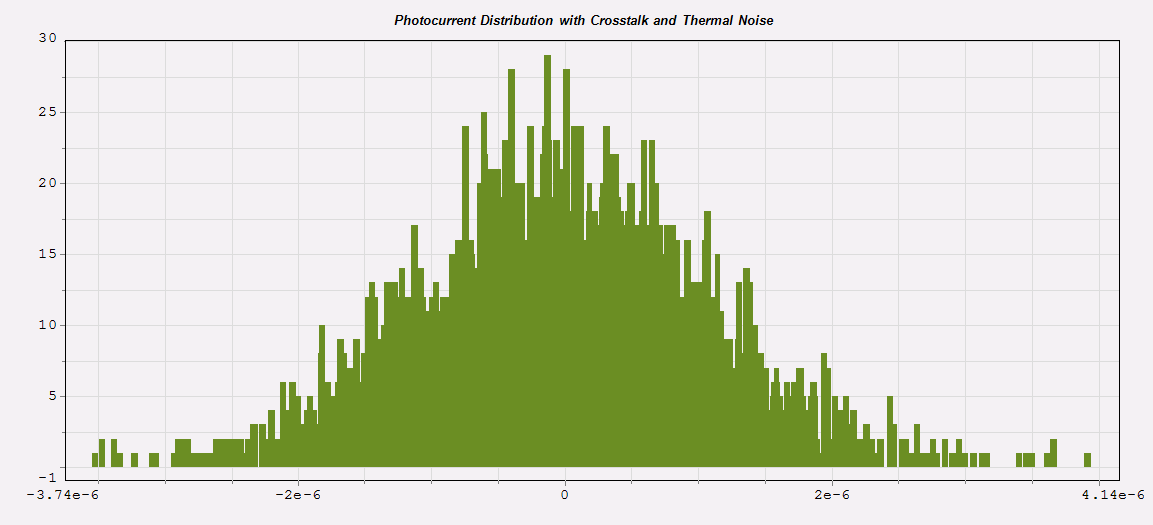
\includegraphics[width=11cm]{ex3_2.png}\\
   \caption{Histogram, L=100 Km.}
   \label{ex3_2}
\end{figure}

We set now the extinction ratio to 15 dB: the estimated BER is $3.01 \cdot 10^{-2}$, in Figure \ref{ex3_3} is shown the histogram.
By lowering the extinction ratio, the BER increases.

\begin{figure}[!ht]
   \centering
   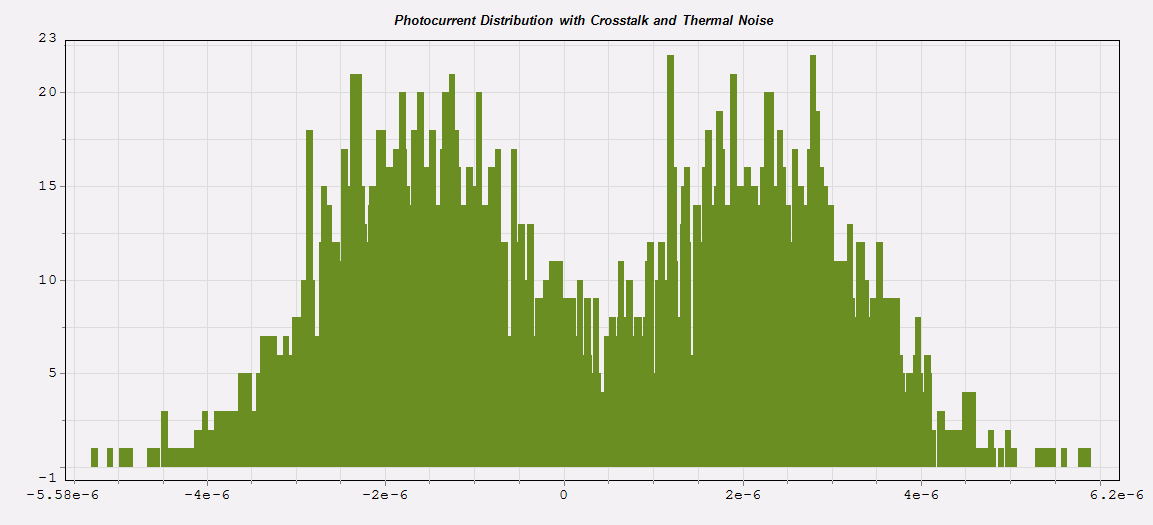
\includegraphics[width=11cm]{ex3_3.png}\\
   \caption{Histogram, extinction ratio = 15 dB.}
   \label{ex3_3}
\end{figure}

We can conclude that, by increasing the transmitted power, the BER decreases as a stronger signal reaches the photodetector and
so the discrimination is easier.
By increasing the length of the link the BER worsens (it increases) as the attenuation is higher and the discrimination is more difficult.
By increasing the extinction ratio (that is the ratio of the power of the bit ``1'' on the power of the bit ``0'')
the discrimination is more easy and so the BER decreases.

\newpage
%%%%%%%%%%%%%%%%%%%%%%%%%%%%%%%%%%%%%%%%%%%%%%%%%%%%%%%%%%%%%%%%%%%%%%%%%%%%%%%%%%%%%%%%%%%%%
\section*{Exercise 4}
We investigate the dependence of the estimated BER on the number of bits used in the estimation. For each sample size the simulation
is iterated 10 times in order to reveal the fluctuations in the estimation of the Q and of the BER. These fluctuations are due to the
randomness of the PRBS sequence as well as the nature of the Q and BER estimation.
We set the power to 1 mW and we vary the number of bits in the PRBS sequence simulated by the setup.
In Figure \ref{ex4_1} and \ref{ex4_2} are shown the plots of the BER (in logarithmic scale) and of the Q versus the number of iterations.
It is possible to observe that, increasing the number of bits in the sequence, the fluctuations in the BER and in the Q decrease.

\begin{figure}[!ht]
   \centering
   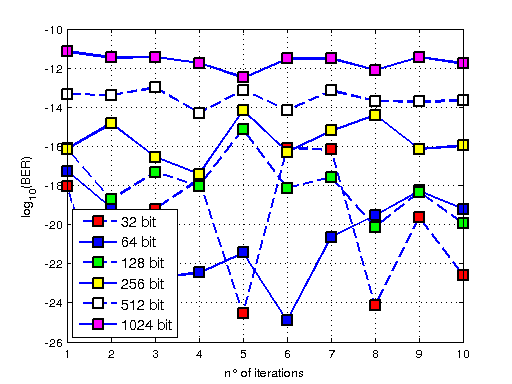
\includegraphics[width=11cm]{ex4_1.png}\\
   \caption{BER versus number of iterations.}
   \label{ex4_1}
\end{figure}

\begin{figure}[!ht]
   \centering
   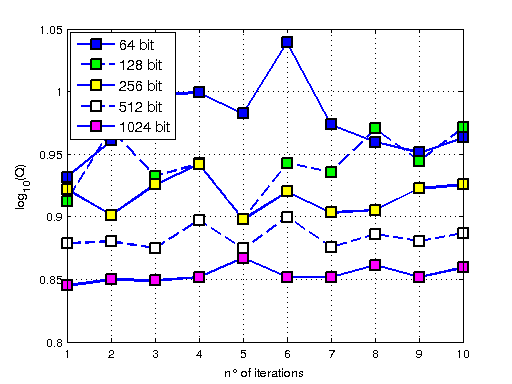
\includegraphics[width=11cm]{ex4_2.png}\\
   \caption{Q versus number of iterations.}
   \label{ex4_2}
\end{figure}

We compute the maximum deviation of BER and Q versus the sample size.
The maximum deviation is obtained by taking the difference between the maximum and the minimum value of each sample size
(that is the maximum and the minimum over the 10 iterations).
In Figure \ref{ex4_3} is shown the plot relative at the BER, while in Figure \ref{ex4_4} is shown the plot relative at the Q.

\begin{figure}[!ht]
   \centering
   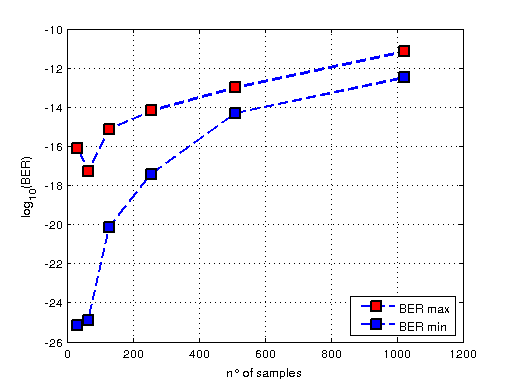
\includegraphics[width=11cm]{ex4_3.png}\\
   \caption{BER maximum and minimum deviation.}
   \label{ex4_3}
\end{figure}

\begin{figure}[!ht]
   \centering
   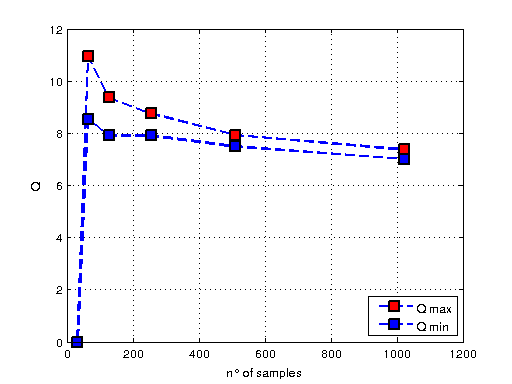
\includegraphics[width=11cm]{ex4_4.png}\\
   \caption{Q maximum and minimum deviation.}
   \label{ex4_4}
\end{figure}


\newpage
%%%%%%%%%%%%%%%%%%%%%%%%%%%%%%%%%%%%%%%%%%%%%%%%%%%%%%%%%%%%%%%%%%%%%%%%%%%%%%%%%%%%%%%%%%%%%
\section*{Exercise 5}
The simulation consists of a transmitter that is an externally modulated laser, and a receiver that is a PIN photodiode with responsivity 1 [A/W].
We measure the BER of the received signal by clock recovery statistical method. Input power is measured by a power meter.
We increase the attenuator loss from 26 to 35 dB, with steps of 1 dB. In Figure \ref{ex5_1} is shown the plot of the logarithm
of the BER versus input power (that is we plot $-\log(-\log(BER))$).
We can observe that the BER linearly decreases as the input power increases.
We can compute the receiver sensitivity by looking at the power value in correspondence of a BER of $10^{-9}$. As we use a logarithmic scale,
we zoom the graph and we read the value that corresponds at $-\log_{10}(9)=-0.9542$.
In Figure \ref{ex5_2} is shown the result: the obtained curve is a line and the sensitivity is about -32.4 dBm.

\begin{figure}[!ht]
   \centering
   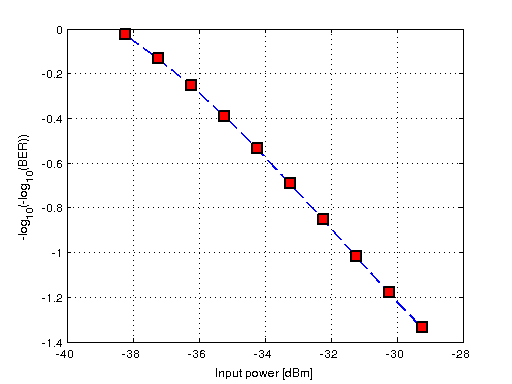
\includegraphics[width=11cm]{ex5_1.png}\\
   \caption{BER versus input power.}
   \label{ex5_1}
\end{figure}

\begin{figure}[!ht]
   \centering
   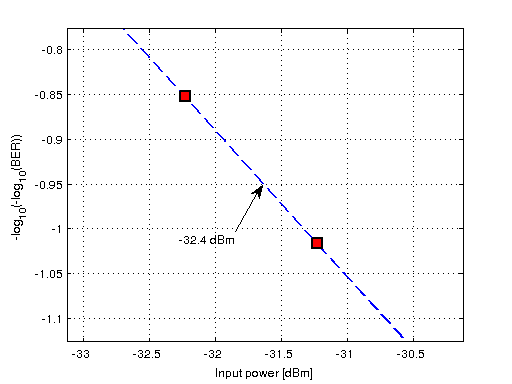
\includegraphics[width=11cm]{ex5_2.png}\\
   \caption{Receiver sensitivity.}
   \label{ex5_2}
\end{figure}

Now we vary the responsivity and we run the simulation again. In Figure \ref{ex5_3} is shown the result.
We can observe that, as the responsivity increases, the BER decreases.

\begin{figure}[!ht]
   \centering
   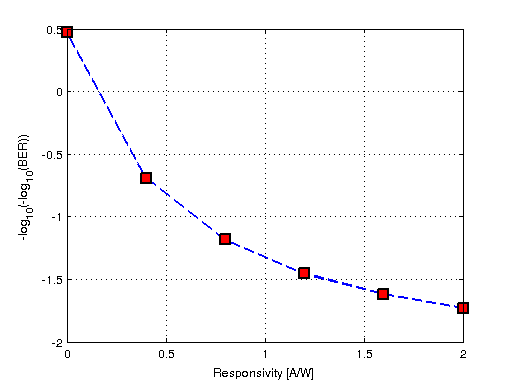
\includegraphics[width=11cm]{ex5_3.png}\\
   \caption{BER versus responsivity.}
   \label{ex5_3}
\end{figure}



\newpage
%%%%%%%%%%%%%%%%%%%%%%%%%%%%%%%%%%%%%%%%%%%%%%%%%%%%%%%%%%%%%%%%%%%%%%%%%%%%%%%%%%%%%%%%%%%%%
\section*{Exercise 6}
Now we test 50 Km of fiber. We vary the attenuator loss from 16 to 21 dB, with steps of 1 dB and we plot the relative BER curve.
In Figure \ref{ex6_1} is shown the result: the obtained curve is a line.

\begin{figure}[!ht]
   \centering
   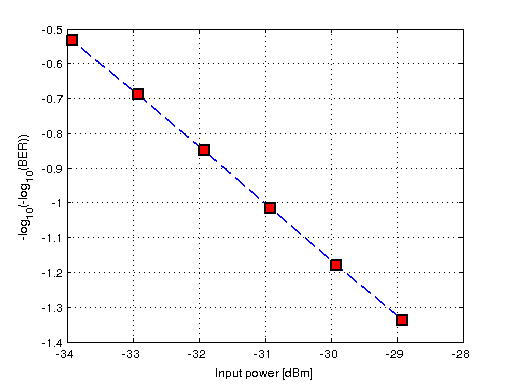
\includegraphics[width=11cm]{ex6_1.png}\\
   \caption{BER versus input power.}
   \label{ex6_1}
\end{figure}

We compare this result with the one obtained by using the back-to-back measurement. In Figure \ref{ex6_2} is shown the result.
We can notice that the curve obtained by using the 50 Km optical fiber is shifted respect to the one of the back-to-back measurement.
The difference in power between the two curves when the BER is $10^{-9}$, that is the power penalty, is about 0.3 dB.
In Figure \ref{ex6_3} is shown the measure.

\begin{figure}[!ht]
   \centering
   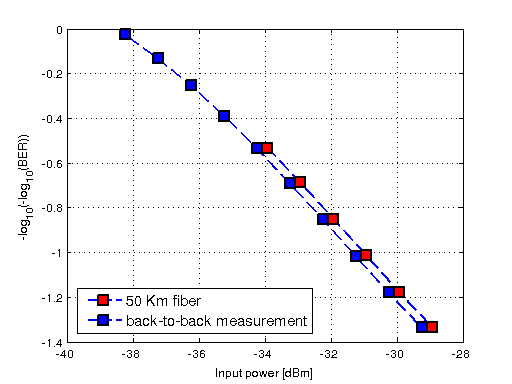
\includegraphics[width=11cm]{ex6_2.png}\\
   \caption{BER versus input power, comparison.}
   \label{ex6_2}
\end{figure}

\begin{figure}[!ht]
   \centering
   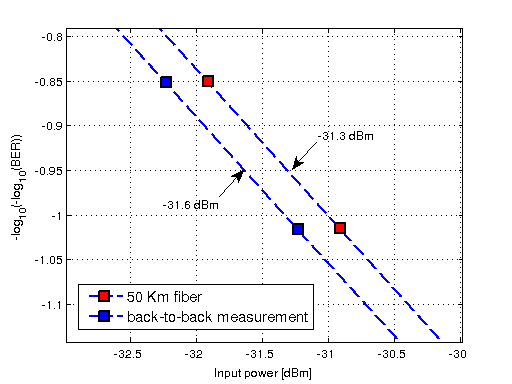
\includegraphics[width=11cm]{ex6_3.png}\\
   \caption{Power penalty.}
   \label{ex6_3}
\end{figure}

\newpage
Now we change the fiber length and we run the simulation again: in Figure \ref{ex6_4} is shown the plot of the power penalty versus
the fiber length.

\begin{figure}[!ht]
   \centering
   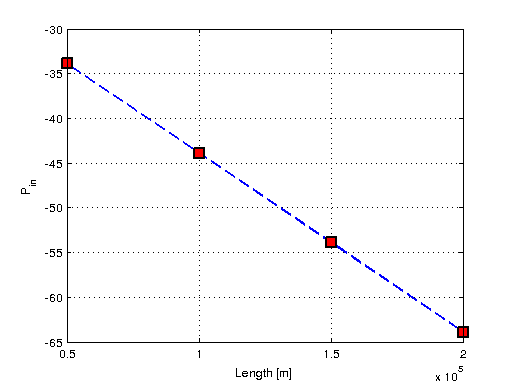
\includegraphics[width=11cm]{ex6_4.png}\\
   \caption{Input power versus length.}
   \label{ex6_4}
\end{figure}

We repeat the experiment (we vary the attenuation loss from 16 to 21 dB), but with the extinction ratio set to 10 dB, instead of 30 dB.
In Figure \ref{ex6_5} is shown the comparison of the obtained graph with the one with an extinction ratio of 30 dB.
We can observe that, if the extinction ratio is higher, the curve BER versus length is shifted down: this means that the BER is lower.
In fact, a higher extinction ratio means a better discrimination between the ``1'' and ``0'' power levels.

\begin{figure}[!ht]
   \centering
   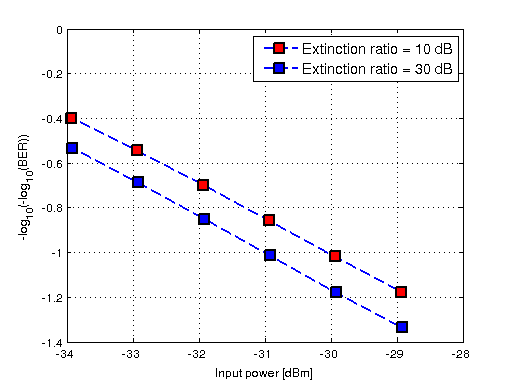
\includegraphics[width=11cm]{ex6_5.png}\\
   \caption{Input power versus length, comparison.}
   \label{ex6_5}
\end{figure}




\newpage
%%%%%%%%%%%%%%%%%%%%%%%%%%%%%%%%%%%%%%%%%%%%%%%%%%%%%%%%%%%%%%%%%%%%%%%%%%%%%%%%%%%%%%%%%%%%%
\section*{Question 3}
By looking at the graphs in Figure \ref{ex6_5}, we can observe that a higher extinction ratio causes a shift in the BER curve.
In fact, the extinction ratio is the ratio between the power of the ``1'' signal on the ``0'' signal.
If this parameter decreases, it means that the distance between the signals ``1'' and ``0'' is lower and so, the discrimination is more
difficult and this translates into a higher BER.



%%%%%%%%%%%%%%%%%%%%%%%%%%%%%%%%%%%%%%%%%%%%%%%%%%%%%%%%%%%%%%%%%%%%%%%%%%%%%%%%%%%%%%%%%%%%%
\section*{Exercise 7}
We test an optically amplified link composed of two parts: one is a back-to-back measurement and the other is an
optically-amplified link measurement, which consists of an optical fiber, an optical amplifier and an optical filter.
We increase the attenuator loss from 0 up to 15 dB, with steps of 1 dB. The link length is 200 Km.

In Figure \ref{ex7_bb} is shown the graph of the BER versus input power for the back-to-back measurement, while in Figure \ref{ex7_oa}
is shown the graph for the optically amplified link.

\begin{figure}[!ht]
   \centering
   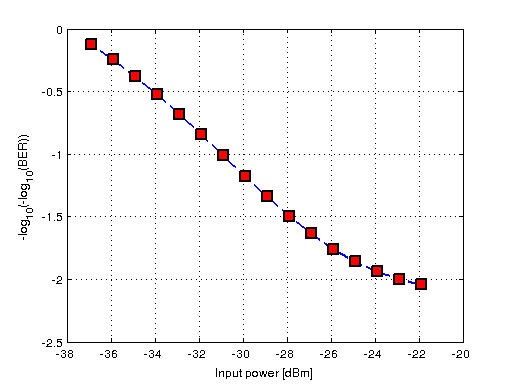
\includegraphics[width=11cm]{ex7_bb.png}\\
   \caption{BER versus input power, back-to-back measurement.}
   \label{ex7_bb}
\end{figure}

\begin{figure}[!ht]
   \centering
   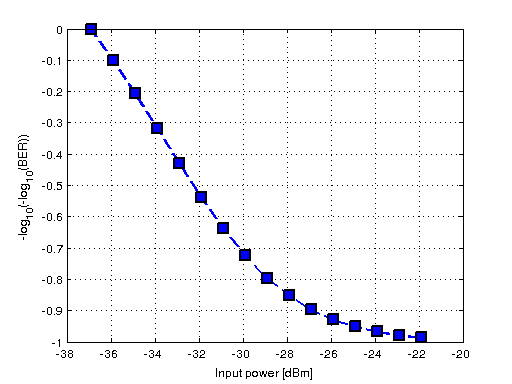
\includegraphics[width=11cm]{ex7_oa.png}\\
   \caption{BER versus input power, optically amplified link.}
   \label{ex7_oa}
\end{figure}

In Figure \ref{ex7_penalty} is shown the comparison between the two curves: the power penalty is 6.4 dBm.

\begin{figure}[!ht]
   \centering
   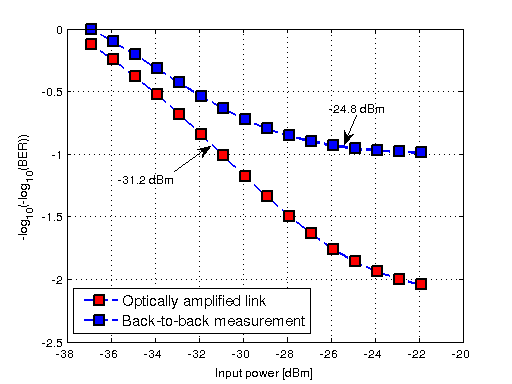
\includegraphics[width=11cm]{ex7_penalty.png}\\
   \caption{Power penalty L=200 Km, G=20 dB.}
   \label{ex7_penalty}
\end{figure}

We change the fiber length to 190 Km and we run the simulation again. In Figure \ref{ex7_penalty190km} is shown the result: the
power penalty is 1.15 dBm.

\begin{figure}[!ht]
   \centering
   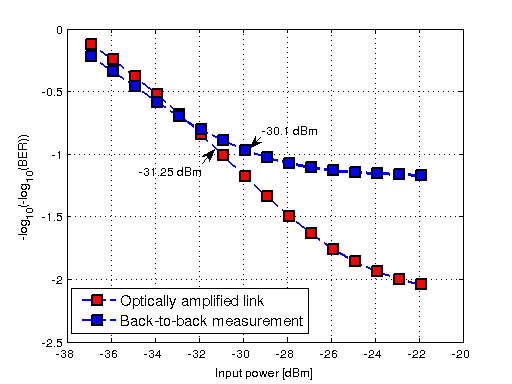
\includegraphics[width=11cm]{ex7_penalty190km.png}\\
   \caption{Power penalty, L=190 Km.}
   \label{ex7_penalty190km}
\end{figure}

We run another simulation with a length of 180 Km, in Figure \ref{ex7_penalty180km} is shown the result: the power penalty is -1.8 dBm.
\begin{figure}[!ht]
   \centering
   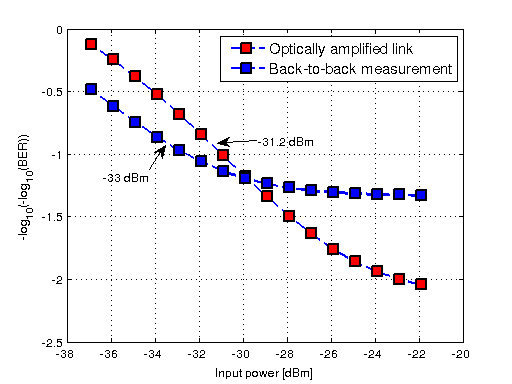
\includegraphics[width=11cm]{ex7_penalty180km.png}\\
   \caption{Power penalty, L=180 Km.}
   \label{ex7_penalty180km}
\end{figure}


\newpage
%%%%%%%%%%%%%%%%%%%%%%%%%%%%%%%%%%%%%%%%%%%%%%%%%%%%%%%%%%%%%%%%%%%%%%%%%%%%%%%%%%%%%%%%%%%%%
\section*{Exercise 8}
We change the gain of the optical amplifier to 18 dB. In Figure \ref{ex7_penalty18dB} is shown the result, the power penalty is 8.25 dBm.

\begin{figure}[!ht]
   \centering
   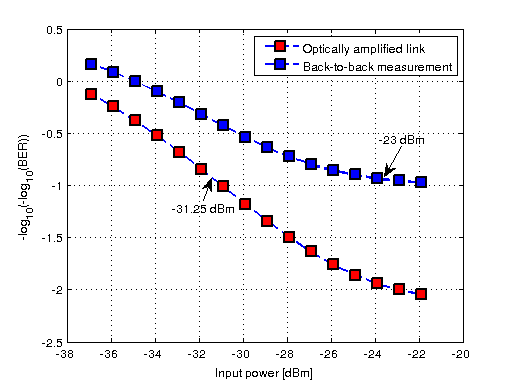
\includegraphics[width=11cm]{ex7_penalty18dB.png}\\
   \caption{Power penalty, P=18 dB.}
   \label{ex7_penalty18dB}
\end{figure}

We decrease the gain to 16 dB and we run another simulation: in Figure \ref{ex7_penalty16dB} is shown the result.
The power penalty is 10 dBm.

\begin{figure}[!ht]
   \centering
   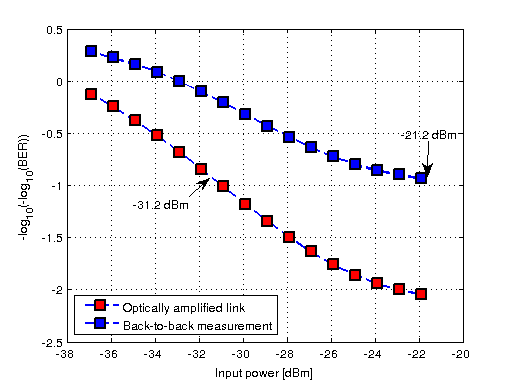
\includegraphics[width=11cm]{ex7_penalty16dB.png}\\
   \caption{Power penalty, P=16 dB.}
   \label{ex7_penalty16dB}
\end{figure}


\newpage
In Table \ref{penalties} is shown the summary of the power penalties obtained by varying the parameters length and gain.
\begin{table}[ht!]
  \begin{center}
    \begin{tabular}{|c|c|c|}
      \specialrule{.1em}{.05em}{.05em}
	 Length [Km] & Gain [dB] & Penalty [dBm] \\
	\hline
	200 & 20 & 6.4\\
	\hline
	190 & 20 & 1.15\\
	\hline
	180 & 20 & -1.8\\
	\hline
	200 & 18 & 8.25\\
	\hline
	200 & 18 & 10\\
      \specialrule{.1em}{.05em}{.05em}
    \end{tabular}
  \end{center}
\caption{Power penalties.}
\label{penalties}
\label{tab}
\end{table}

We plot the penalties respect to the length and to the gain.
In Figure \ref{ex7_penaltycomparison} is shown the plot of the power penalty versus the length.
We can observe that the relation is approximately linear: increasing the length the power penalty linearly increases.

\begin{figure}[!ht]
   \centering
   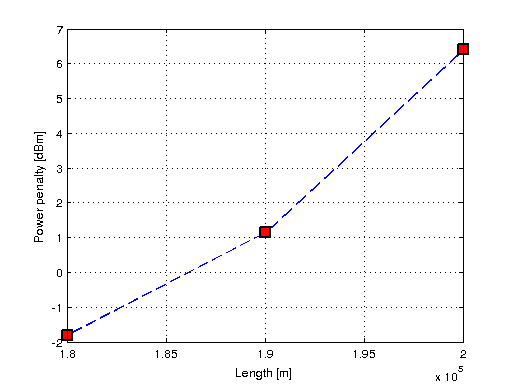
\includegraphics[width=11cm]{ex7_penaltycomparison.png}\\
   \caption{Power penalty versus length.}
   \label{ex7_penaltycomparison}
\end{figure}

In Figure \ref{ex7_penaltycomparison2} is shown the plot of the power penalty versus the gain.
In this case we obtain an inverse linear relation: increasing the gain, the power penalty decreases.

\begin{figure}[!ht]
   \centering
   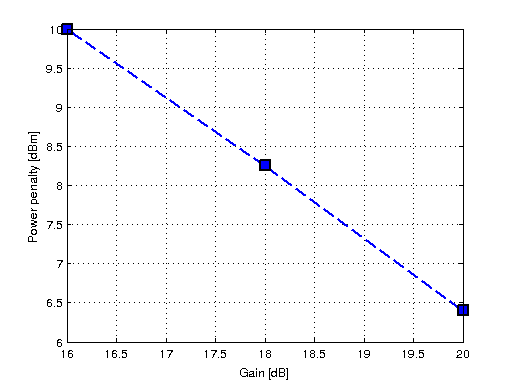
\includegraphics[width=11cm]{ex7_penaltycomparison2.png}\\
   \caption{Power penalty versus gain.}
   \label{ex7_penaltycomparison2}
\end{figure}


\newpage
%%%%%%%%%%%%%%%%%%%%%%%%%%%%%%%%%%%%%%%%%%%%%%%%%%%%%%%%%%%%%%%%%%%%%%%%%%%%%%%%%%%%%%%%%%%%%
\section*{Question 4}
We compare the sensitivity of a PIN diode receiver with the one of an optically amplified PIN diode receiver.
In the schematic, one part is a BER measurement using a normal PIN diode receiver, the other part instead consists of a BER measurement
using an optically pre-amplified receiver, which includes an optical amplifier, an optical filter and a PIN diode receiver.

We set the gain parameter to 20 dB and we vary the attenuation from 28 to 52 dB, in steps of 6 dB.
In Figure \ref{q4} are reported the graphs of the BER versus input power, for the normal receiver and for the optically pre-amplified one.

\begin{figure}[!ht]
   \centering
   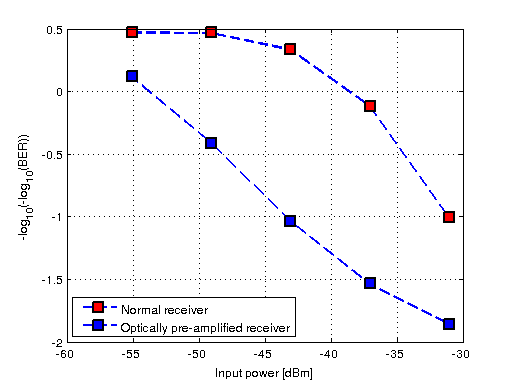
\includegraphics[width=11cm]{q4.png}\\
   \caption{BER versus input power.}
   \label{q4}
\end{figure}

We can observe that the gradient of the two curves is different.
In the case of a normal receiver, the optical power is converted into current fluctuations and to this new current signal
are added shot noise and thermal noise, introduced by the receiver itself. This causes the curve to have a downward concavity with high BER values.

In the case of the optically pre-amplified receiver, instead, the power that reaches the photodetector is higher and consequently,
the current signal generated is higher too and the noise introduced by the photodetector is less significant.
So the BER curve has an upward concavity: it rapidly decreases when the input power increases. 











\end{document}